\documentclass[a4paper,10pt]{report}
\usepackage[utf8]{inputenc}
\usepackage[margin=2.4cm]{geometry}
\usepackage{caption}
\usepackage{wrapfig}
\renewcommand*\thetable{\Roman{table}}
\usepackage[nolists,tablesfirst]{endfloat}
\usepackage{tikz}
\usepackage{placeins}
\usepackage{lscape}
\usepackage{amsmath}
\usepackage{SIunits}
\usepackage{graphicx}
\usepackage{multirow}
\usepackage{multicol}
\usepackage[numbers]{natbib}
\usepackage{blkarray}
\usepackage{rotating}
\usepackage{overpic}
\usepackage{subcaption}
\usepackage{floatrow}
\usepackage{setspace}
\usepackage{authblk}
\usepackage{listings}
\usepackage{textcomp}
\usepackage{color}

\definecolor{dkgreen}{rgb}{0,0.6,0}
\definecolor{gray}{rgb}{0.5,0.5,0.5}
\definecolor{mauve}{rgb}{0.58,0,0.82}
\usepackage[final,colorlinks=true,pdfborder={0 0 0},bookmarksopen=true,bookmarksnumbered=true]{hyperref}

\author[1,2]{Thomas Pfau}

\affil[1]{Life Sciences Research Unit, University of Luxembourg}

\title{Encrypting File Systems with encFS}


\lstset{frame=tb,
  language=bash,
  aboveskip=3mm,
  belowskip=3mm,
  showstringspaces=false,
  columns=flexible,
  basicstyle={\small\ttfamily},
  numbers=none,
  numberstyle=\tiny\color{gray},
  keywordstyle=\color{blue},
  commentstyle=\color{dkgreen},
  stringstyle=\color{mauve},
  breaklines=true,
  breakatwhitespace=true,
  tabsize=3
}






\begin{document}

\begin{titlepage} \begin{center} 
% Title 
~\\[0.4cm] { \huge \bfseries Encryption with encFS \\[0.4cm] } ~\\[1.5cm] 
%\noindent \begin{minipage}[t]{\textwidth} 
\begin{center} 

\large {Thomas Pfau\,$^{a}$}
\end{center} 
\begin{center} 
$^{a}$Life Science Research Unit, University of Luxembourg, Campus Belval, Biotech II, 6 avenue du Swing, L-4367 Belvaux, Luxembourg\\
\end{center}
%\end{minipage}
\vfill % Bottom of the page 
{\large \today} 
\end{center} 
\end{titlepage}

%\subsection{The IDARE Cytoscape app}
\chapter{Installing and using encfs}

Encrypting files containing personal data has become paramount with the introduction of the GDPR.
An simple tool to achieve this is the open Source software encfs, which generates an encrypted file system, and makes it available as an additional Mount point or volume.
While it is easy to use on the command line, a graphical user interface might be preferred by many. 
For windows a GUI exists, in the form of \href{https://github.com/jetwhiz/encfs4win}{encFS4Win}.
However, for Linux and mac, the available tools are not reliable.
Here are instructions on how to use encFS on the different operating systems. How to install it etc. 


\section{Windows}
\subsection{Installation}
The Windows installation file can be found on ATLAS (ATLAS \textrightarrow ENCRYPTION \textrightarrow Windows).\newline
Simply double click the file and install the tool (along with all its requirements) using the installer.
\subsection{Usage}
Once installed, you can start the tool by pressing Start and typing encfs, you will see the encfs programm. Just click it.
A tray icon will be created (A small key icon in the lower right side). 
When you right-click on this icon, You will have options to create new storages, and open existing ones. 
Each Volume will be mapped to a drive letter (e.g. E:) that you can choose. 
While you can have multiple mounts pointing to the same drive letter, they cannot be active simultaneously.

\section{Unix Systems}

\subsection{Installation}
\subsubsection{Mac}
These instructions are for High Sierra (macOS 10.13), but they should work as well for other macOS versions.
You will need to install the encfs tool and java before you can start. To do so, we will install Homebrew (if it is not yet installed), which makes the installation much easier
Run the following command in a terminal (LaunchPad \textrightarrow Other/Utilities \textrightarrow Terminal):
\begin{lstlisting}
ruby -e "$(curl -fsSL https://raw.githubusercontent.com/Homebrew/install/master/install)"
\end{lstlisting}
First, we will install java using homebrew:
\begin{lstlisting}
brew cask install java
\end{lstlisting}
encfs requires the FUSE (Filesystem in USErspace) package to work, so we will install it as 
\begin{lstlisting}
brew cask install osxfuse
\end{lstlisting}
And finally install encfs as:
\begin{lstlisting}
brew install encfs
\end{lstlisting}



\subsubsection{Linux}
We assume you are on an apt-based system (our example is for ubuntu 16.04). If you are using a different package manager, you will have to adapt the instructions accordingly.
\subsection{Installation}
You will need to install encfs and java.
\begin{lstlisting}
 sudo apt-get install encfs
 sudo apt-get install default-jdk
\end{lstlisting}
After these installations, you can copy the Jar file from ATLAS \textrightarrow ENCRYPTION \textrightarrow Linux to your machine.
Run the jar file (either by double-click (if your settings are set up to run jar files) or by ``right click'' \textrightarrow ``open with'' \textrightarrow ``(Open)JDK ..''

\subsection{Usage}
After starting the application, you will see the interface shown in Figure \ref{interface}.
\begin{wrapfigure}{R}{0.4\textwidth}
 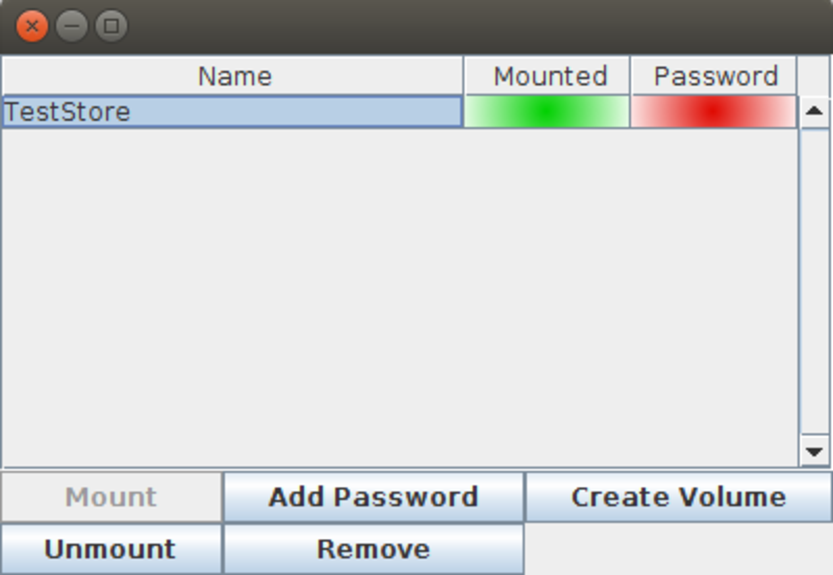
\includegraphics[width=\textwidth]{Docu/Interface}
  \caption{The interface of the tool, each store is displayed in an individual row, and its activity status is indicated.}
  \label{interface}
\end{wrapfigure}
You can create new encrypted volumes and mount/unmount volumes  using this interface. This is also posible by using the tray icon generated.
Closing the Interface does not close the tool! IT will stay open as tray icon, and you can reopen the Interface by right-clicking on the tray icon and select ``Open Manager''.
Only if you exit from the tray icon, the tool will shut down.
If you do so, all your mounts will be unmounted (disconnected), and you will need to reopen them, if you want to use them again.
\subsection{Password storage}
The tool offers a password storage, so that you don't need to remember all passwords for the different storages. If using this feature, please use a strong master password to protect them.
The first time you cick ``Add Password'', you will be asked to set up a master password. The master password cannot be changed (at the moment). 
If you want to access a volume for which you have saved a password, you will be asked to provide the master key to unlock the stored password. 
A entered master key will be remembered for about 5 minutes, i.e. any other volumes you open in this time which have stored passwords will not require you to enter a password.


\end{document}
